\documentclass[10pt, a4paper]{article}


\usepackage{graphicx}
\usepackage{amsmath}
\usepackage{subcaption}
\usepackage{float}
\usepackage{hyperref}
\usepackage[margin=0.5in]{geometry}

\begin{document}
    
\title{MATH 310: Probability \& Statistics \\Project Report}
\author{Owais Bin Asad, Aaron Lucas Soares, Bahzad Ahmed Badvi}

\maketitle

\section*{Github Repository}
The Github repository can be accessed and cloned at: \href{https://github.com/doodhJalebi/Prob-Stat---Project-Spring-2020-}{https://github.com/doodhJalebi/Prob-Stat---Project-Spring-2020-}.

\section*{Task 1}
\subsection*{Simulation Model:}
In order to determine a good average distance from starting position for each step number, the simulation was run
100 times, each one being 1000 steps long. The resulting model gives us a good idea of what the
distance from the starting point would be given that $n$ number of steps have elapsed. Refer to figure 1.

\subsection*{Mathematical Model:}
\begin{align*}
    y_{t+1} = y_{t} + X
\end{align*}

where X is a discrete random variable that takes on discrete values $[-1, 1]$ with probabilites $[0.5, 0.5]$ respectively.
$y_t$ is the distance from the starting point at time $t$. $y_{t+1}$ is the distance from the starting point at time $t+1$.


\section*{Task 2}
\subsection*{Simulation Model:}
In order to determine a good average number of steps for a fixed starting distance between the two persons, the simulation was run
100 times, each one being 1000 steps long, for each value of starting distance $x$. Refer to figure 2.

\subsection*{Mathematical Model:}
\begin{align*}
    E[T] = \frac{1}{2}(\text{time for person A to reach }\frac{d}{2})\text{ for even d}\\
    E[T] = \frac{1}{2}(\text{time for person A to reach }\frac{d+1}{2})\text{ for odd d}\\
\end{align*}

where T is a random variable that denotes the time taken in number of steps for person A and B to meet.
$d$ is the distance between them at time $t = 0$.


\section*{Task 3}
\subsection*{Simulation Model:}
The simulation was run first for a single random walk and then for 100 random walks in order to observe the differences and randomness in the walks. The simulation with the nodes having an equal probability to move in discrete values for angles and step size. No pattern could be observed from this. However, when running the simulation with unequal probabilities for angles and step size, a pattern could be found in which all random walks were simulated close to each other, at the angle having the highest probability.
Refer to figures 3 and 4.

\subsection*{Re-entry Model:}
The Re-entry model works by detecting on every step if the next step taken would cross the boundary, if so the particle stays where it is for the step, however it is allow to move in the next step if it isn't crossing the boundary. In order to achieve this we added a check for euclidean distance from the origin and compared with the radius every time a step is taken and work along that. This Re-entry model ensures that the particle does not escape the circle and that it can still move by changing its direction in the upcoming steps.\\
Our choice using such a model was such that we can ensure every step taken is allowed and random.


\section*{Task 4}
\subsection*{Simulation Model:}
This builds on Task 1's simulation model with the only difference being that the step size is modeled by a uniform random variable now.
Refer to figure 5.

\subsection*{Mathematical Model:}
\begin{align*}
    y_{t+1} = y_{t} + X
\end{align*}

where X is a continuous random variable that takes on values $[0, 1]$ with unifrom probabilites.
$y_t$ is the distance from the starting point at time $t$. $y_{t+1}$ is the distance from the starting point at time $t+1$.


\section*{Task 5}
\subsection*{Simulation Model:}
Simulations for Task 5 were conducted in a similar manner to that of Task 3. Instead of using discrete values of angles and step size, continuous values were chosen from the given range. When taking a closer look at the simulation results (zooming in), it could be observed that each step taken by each node was different, as each angle and step size was different. 
Refer to figure 6 and 7.


\section*{Task 7}
\subsection*{Simulation Model:}
Simulations for Task 7 were conducted in a similar manner to that of Task 3. Instead of using discrete values of angles and step size, continuous values were chosen for the angles and discrete values for the step size. When taking a closer look at the simulation results (zooming in), the angles of each step differed from each other but there were similarity in the step sizes since discrete values were used.
Refer to figure 8 and 9.


\section*{Task 8}
\subsection*{Simulation Model:}
In order to make this simulation we ran a simulation similar to Task 5, but now we added two particles to the same space and let them wander through defined protocols until they came closer than $1$ unit between one another. The initial positions were calculated by choosing a distance $r$ and an angle $\theta$ from a uniform continuous sample space of $0-R$, where $R$ is radius and $0-2\pi$ for angle.\\
This simulation was then run for 10 different positions of particles, each run for 10 times, to get a mean value of steps for each of these positions. Then our data was plotted as mean number of steps against the Euclidean distance between particles' initial position.
Refer to figure 10.

\newpage

\section*{Figures}

\begin{figure}[H]
    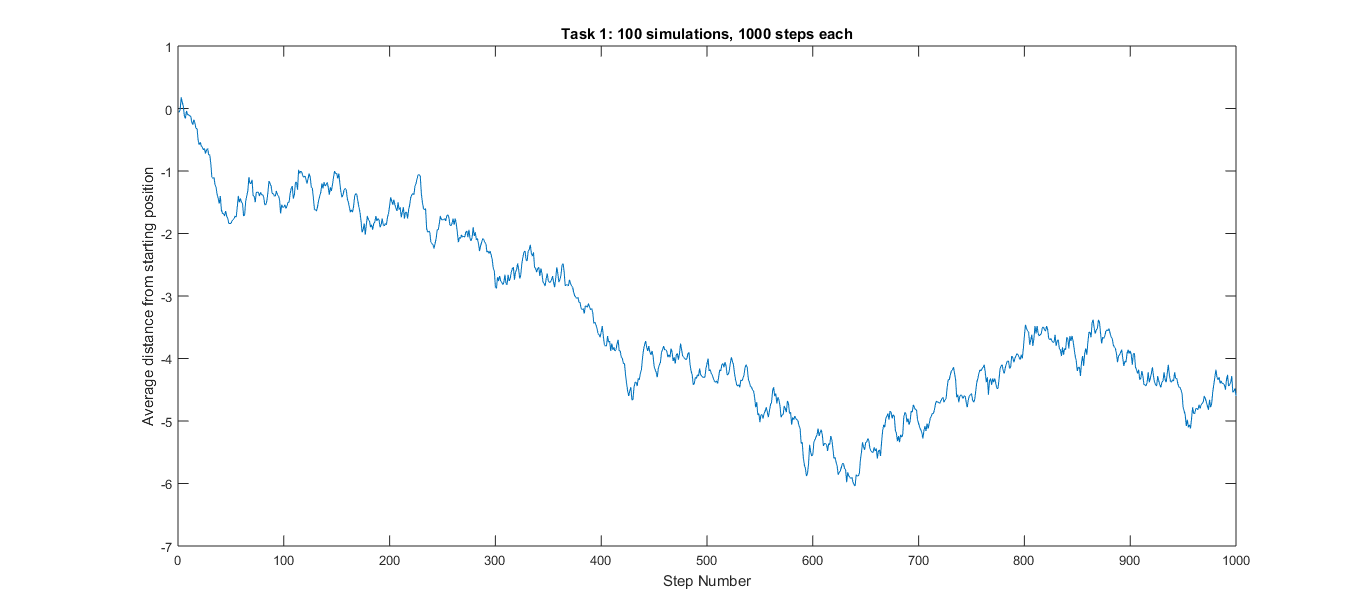
\includegraphics[width=\textwidth]{Diagrams/Task 1 Testing/100 simulations, 1000 steps/graph.png}
    \caption{}
    \label{fig:1}    
  \end{figure}

\begin{figure}[H]
    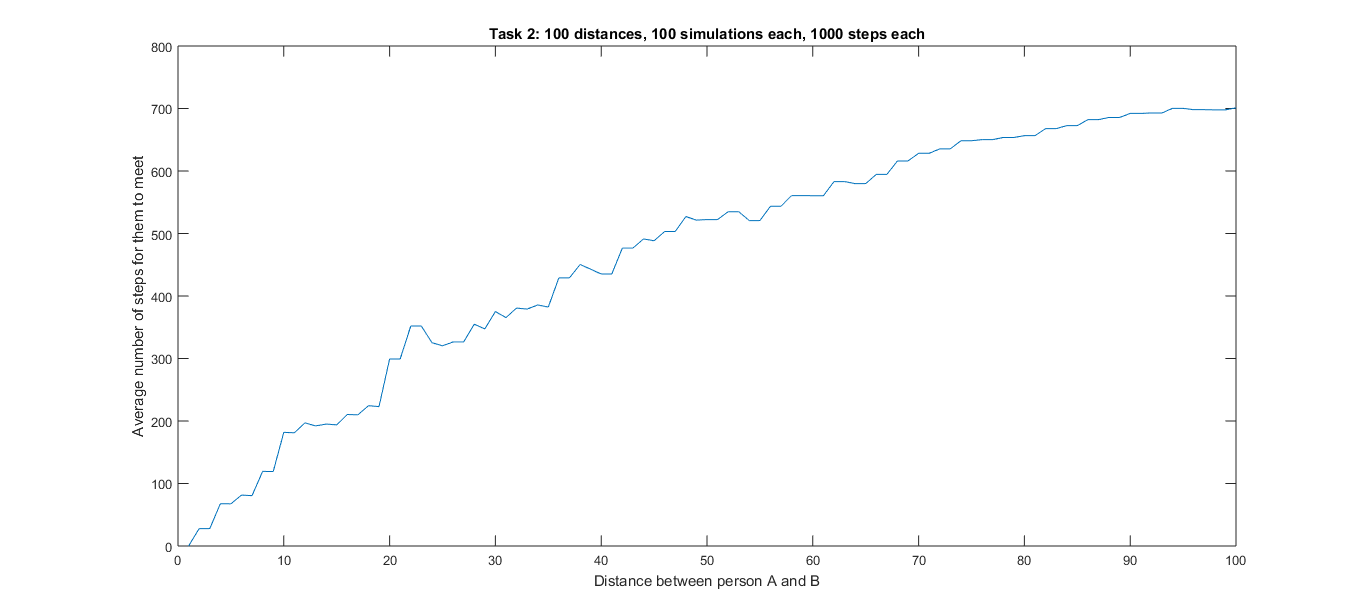
\includegraphics[width=\textwidth]{Diagrams/Task 2 Testing/ureka.png}
    \caption{}
    \label{fig:2}
\end{figure}

\begin{figure}[H]
    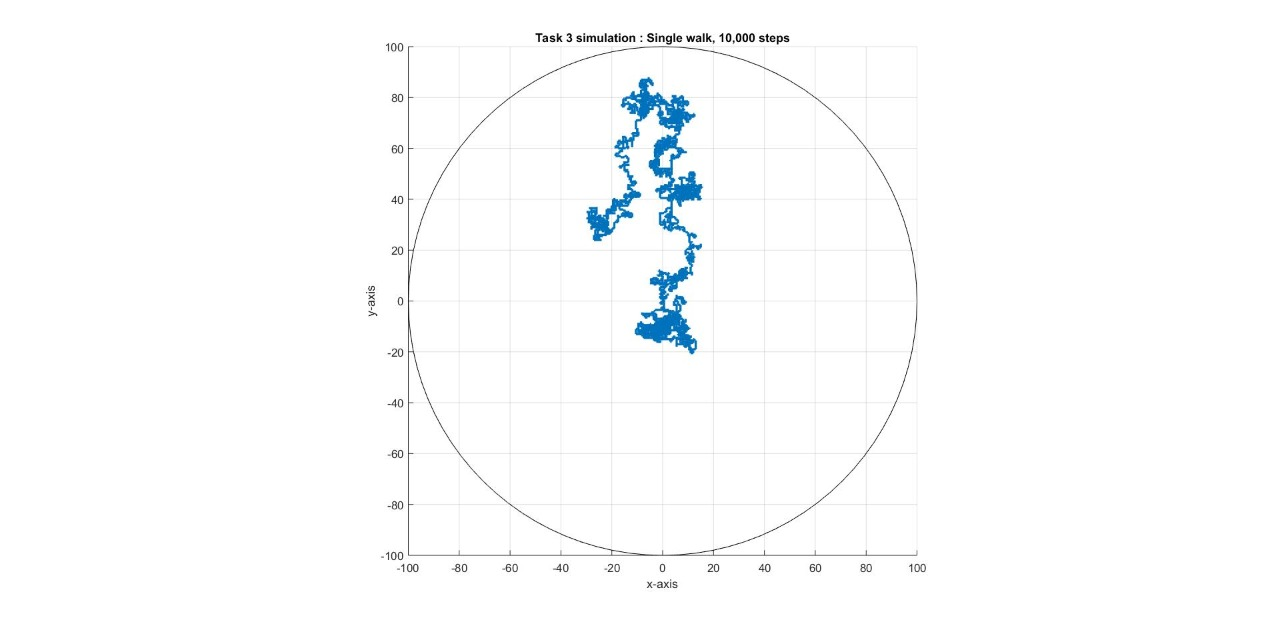
\includegraphics[width=\textwidth]{Diagrams/Task 3 Testing/single_walk_Task_3.jpeg}
    \caption{}
    \label{fig:3}
\end{figure}

\begin{figure}[H]
    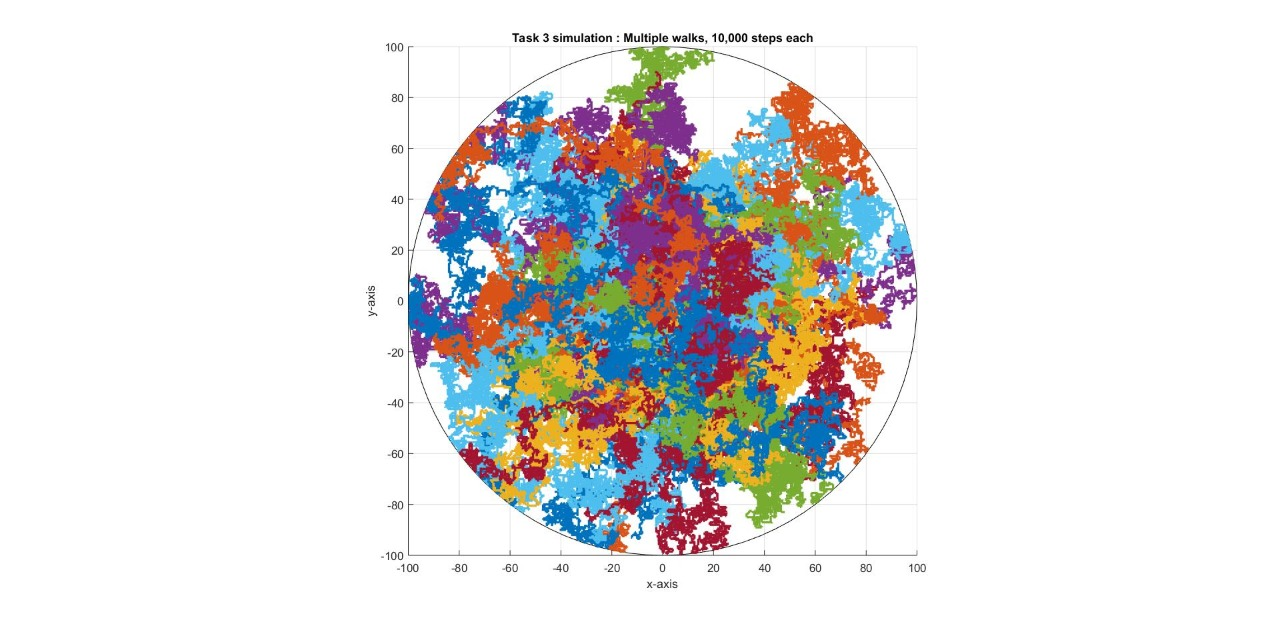
\includegraphics[width=\textwidth]{Diagrams/Task 3 Testing/multiple_walks_Task_3.jpeg}
    \caption{}
    \label{fig:4}
\end{figure}

\begin{figure}[H]
    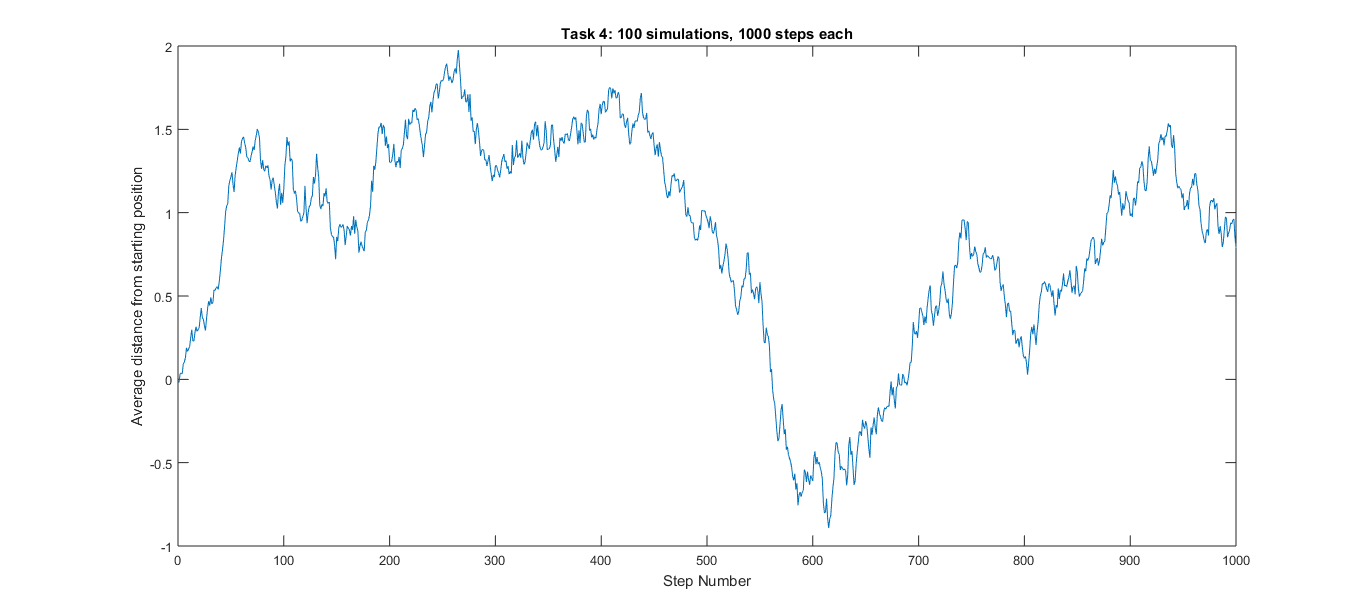
\includegraphics[width=\textwidth]{Diagrams/Task 4 Testing/graph.png}
    \caption{}
    \label{fig:5}
\end{figure}

\begin{figure}[H]
    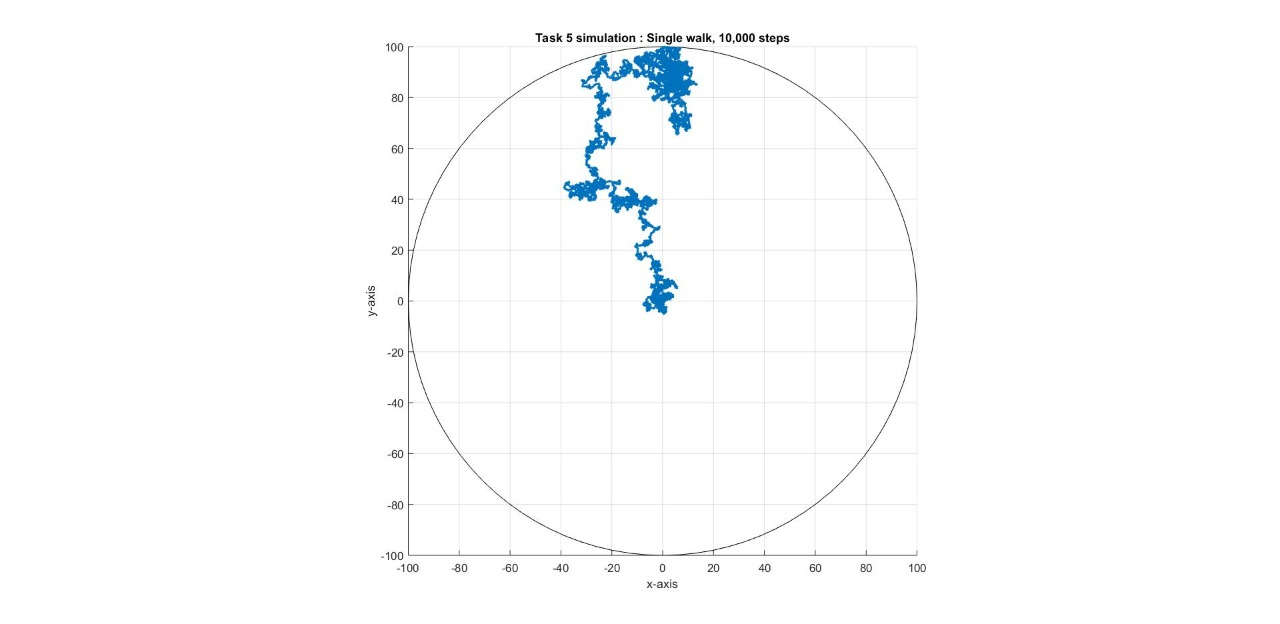
\includegraphics[width=\textwidth]{Diagrams/Task 5 Testing/single_walk_task_5.jpeg}
    \caption{}
    \label{fig:6}
\end{figure}

\begin{figure}[H]
    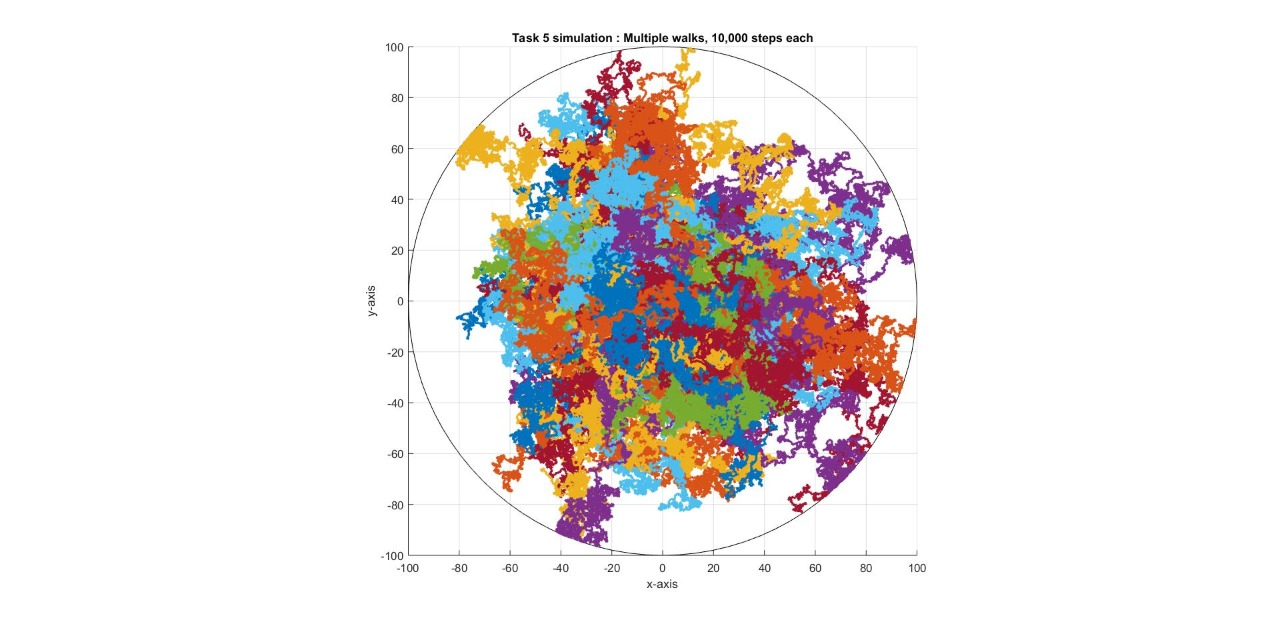
\includegraphics[width=\textwidth]{Diagrams/Task 5 Testing/multiple_walks_task_5.jpeg}
    \caption{}
    \label{fig:7}
\end{figure}

\begin{figure}[H]
    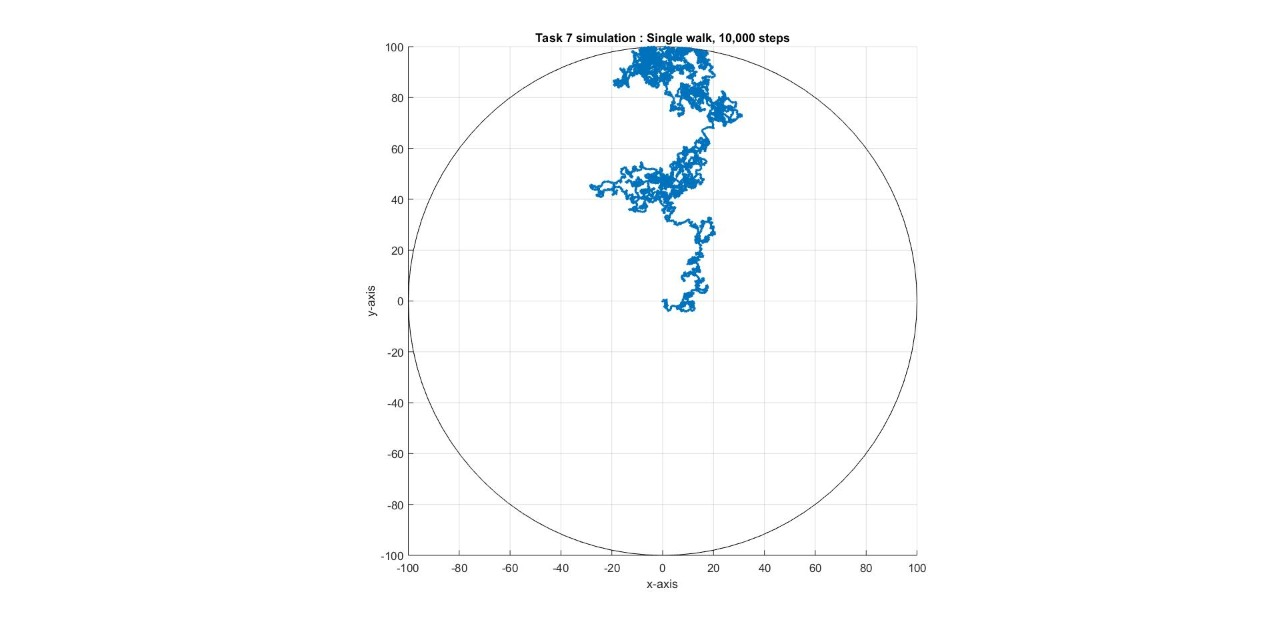
\includegraphics[width=\textwidth]{Diagrams/Task 7 Testing/single_walk_task_7.jpeg}
    \caption{}
    \label{fig:8}
\end{figure}

\begin{figure}[H]
    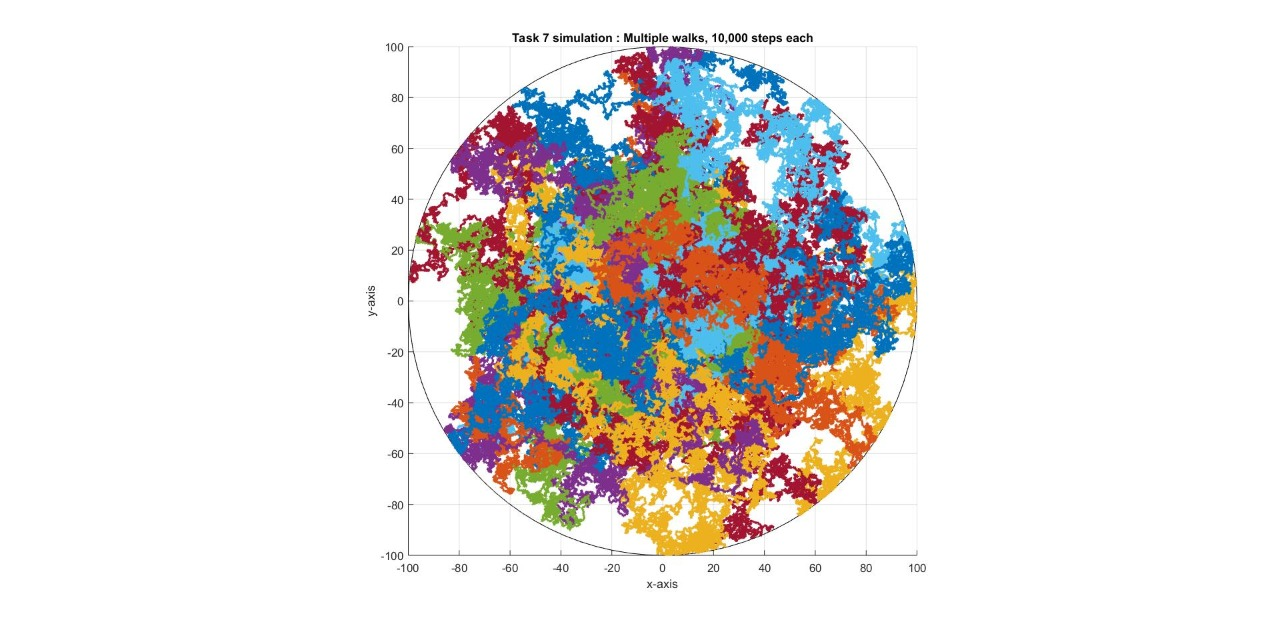
\includegraphics[width=\textwidth]{Diagrams/Task 7 Testing/multiple_walks_task_7.jpeg}
    \caption{}
    \label{fig:9}
\end{figure}

\begin{figure}[H]
    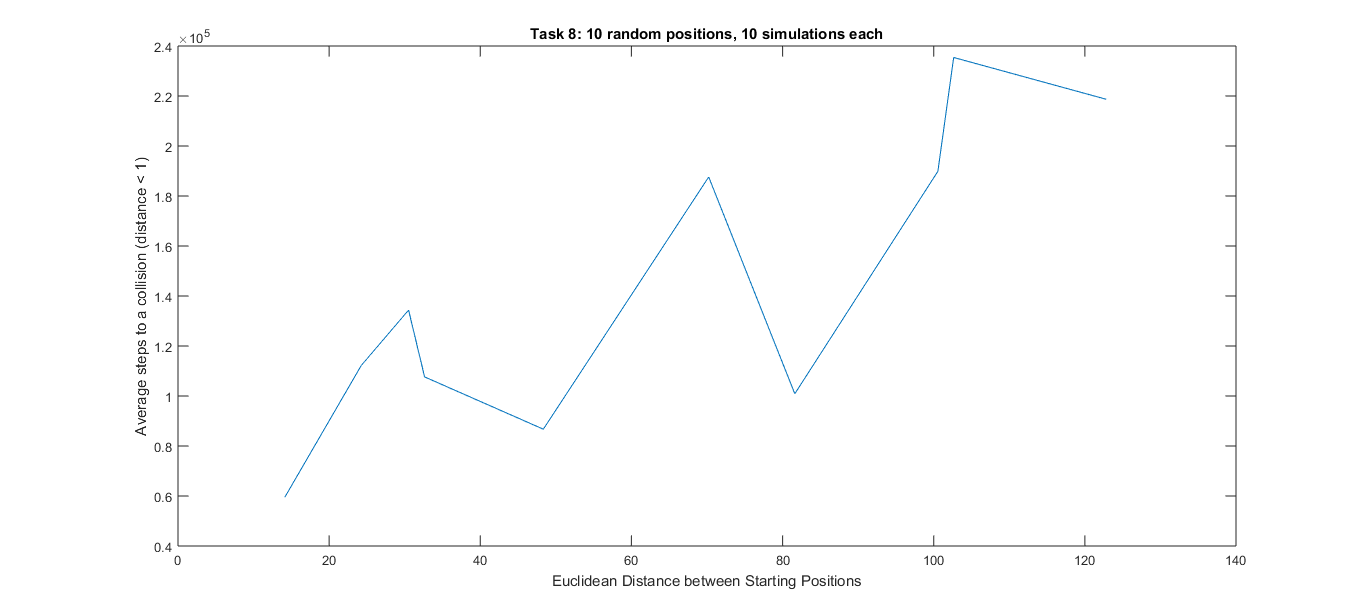
\includegraphics[width=\textwidth]{Diagrams/Task 8 Testing/graph.png}
    \caption{}
    \label{fig:10}
\end{figure}
\end{document}
